\documentclass[10pt,twocolumn,letterpaper]{article}

\usepackage{statcourse}
\usepackage{times}
\usepackage{epsfig}
\usepackage{graphicx}
\usepackage{amsmath}
\usepackage{amssymb}

% Include other packages here, before hyperref.

% If you comment hyperref and then uncomment it, you should delete
% egpaper.aux before re-running latex.  (Or just hit 'q' on the first latex
% run, let it finish, and you should be clear).
\usepackage[breaklinks=true,bookmarks=false]{hyperref}


\statcoursefinalcopy


\setcounter{page}{1}
\begin{document}


%%%%%%%%%%%%%%%%%%%%%%%%%%%%%%%%%%%%%%%%%%%%%%%%%%%%%%%%%%%%%%%
% DO NOT EDIT ANYTHING ABOVE THIS LINE
% EXCEPT IF YOU LIKE TO USE ADDITIONAL PACKAGES
%%%%%%%%%%%%%%%%%%%%%%%%%%%%%%%%%%%%%%%%%%%%%%%%%%%%%%%%%%%%%%%



%%%%%%%%% TITLE
\title{STAT479 Project Proposal}

\author{Tong Li\\
{\tt\small tli287@wisc.edu}
\and
Runxin Gao\\
{\tt\small rgao35@wisc.edu}
\and
Kenny Jin\\
{\tt\small jjin59@wisc.edu}
}

\maketitle
%\thispagestyle{empty}



% MAIN ARTICLE GOES BELOW
%%%%%%%%%%%%%%%%%%%%%%%%%%%%%%%%%%%%%%%%%%%%%%%%%%%%%%%%%%%%%%%



%%%%%%%%% BODY TEXT



\section{Introduction}


Quick, Draw!\footnote{https://quickdraw.withgoogle.com/} is an online game released by Google on November, 2016 where the user is prompted with a specific requirement to draw a picture in 20 seconds and the algorithm will make a prediction based on the drawing. Millions of images were collected by Google through this game, and they were utilized to make better and quicker predictions. Figure \ref{fig:quickdraw} showed an example of such images\footnote{https://github.com/googlecreativelab/quickdraw-dataset}. Such large-scale data set leaves many to the imagination of machine learning enthusiasts and encourages the rises of creative projects. For example, Quartz has explored the drawing habits like stroke order grouped by different countries and found clear associations between the drawing and their language styles \cite{quartzcircle}; others tried several different prediction models evaluated by prediction accuracy \cite{github}.


Inspired by these existing projects, we have three-fold goals for the project. One fundamental objective for this project is to use different machine learning models for accurate image classifications based on the features of the doodles. Therefore, one feasible classification algorithm is the k-Nearest Neighbor (k-NN) method. However, since k-NN can be greatly affected by the curse of dimensionality, and each image in the data set is a 28*28 bitmap, we will need to do dimensionality reduction to make better use of k-NN. And one approach to reduce dimension is probably by Principal Component Analysis (PCA). Another approach that could be used is Random Forest, which is an ensemble method that grows different decision tree models and pruning could be adopted to improve the accuracy. Other possible algorithms that could be used for the classification task are Support Vector Machine (SVM) and Convolutional Neural Networks (CNN).


However, the drawings are not identical in each category and the doodles of different categories may look very similar. For instance, ‘teapot’\footnote{https://quickdraw.withgoogle.com/data/teapot}  category includes many versions of doodles Figure \ref{fig:teapot}, and the drawings from wine bottle and vase categories could be somehow indistinguishable. Therefore, to increase the prediction accuracy, we aim to use the k-means method in each category to create several clusters and then apply k-NN to classified the drawing based on k-nearest centroids, where k is a hyperparameter and could be tuned through methods such as cross validation.


After getting the trained prediction models, we want to compare their prediction accuracy and to analyze their pros and cons. We also want to find corresponding ways to improve the accuracy. 

Besides the prediction models, we also tend to do Exploratory Data Analysis (EDA) on parts of original data set and the simplified one to find hidden relations between features in each drawing category. We might analyze the stroke order and time stamp in each category of pictures and try to summarize the corresponding drawing styles. 




\begin{figure}[h]
\begin{center}
   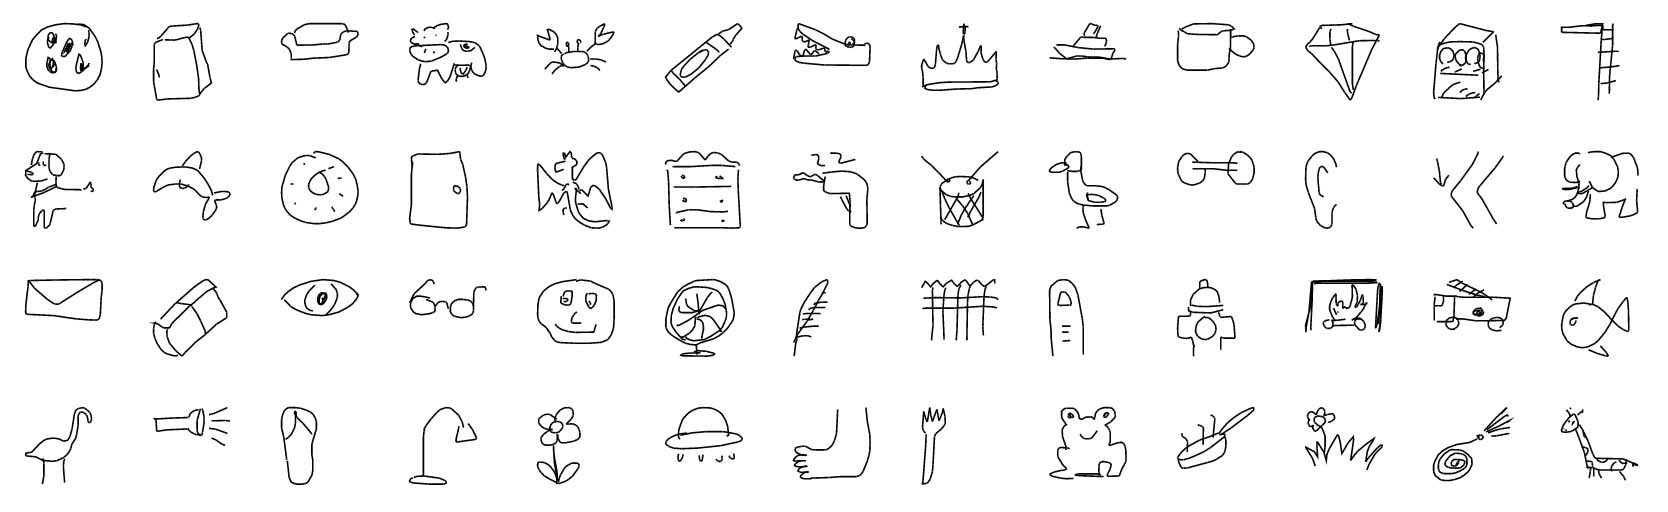
\includegraphics[width=0.8\linewidth]{figures/quickdraw_image.jpg}
\end{center}
   \caption{Example of quick draw imgaes}
\label{fig:quickdraw}
\end{figure}


\begin{figure}[h]
\begin{center}
   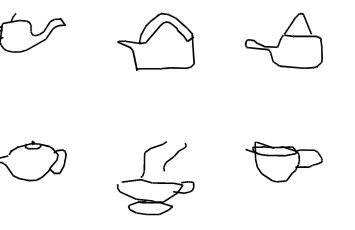
\includegraphics[width=0.8\linewidth]{figures/teapot.png}
\end{center}
   \caption{Example drawings of teapot}
\label{fig:teapot}
\end{figure}

\section{Motivation}

Image classification is an important task in machine learning. While there are various kinds of images, the drawings in the Quick, Draw! dataset is very special. The drawings are already abstractions of entities, and it will be interesting to see different machine learning algorithms perform in this special image dataset.

 
Such algorithms could also have some educational applications. For example, for toddlers who are still learning a language, if we have the algorithms that make accurate predictions based on doodles, then toddlers will be able to draw what they observe and learn how to say or write it, which could accelerate the language learning process. Moreover, since doodles are somewhat sketchy, by constructing algorithms that can make accurate predictions based on sketchy images, the uses of the algorithms could be extended to convert handwritten text to computer, eliminating the need to type all the words again. 

\section{Evaluation}

As all other classification algorithms, accurate classification is the aim and prediction accuracy is the most straightforward measure. Let $A$ be the total number of correctly classified samples, and $T$ be total number of samples, then the  evaluation formula would be: 

\begin{equation}
Accuracy=\frac{A}{T}
\end{equation}

A high accuracy of the prediction could mean the selected model is successful in the prediction of the corresponding category. Also, it might be easier for the model to predict some certain categories more accurately, thus the equation above could also be used for a single category of images.

However, this way of evaluation seems insufficient , because some categories have similar drawings, such as vase and wine bottle. Therefore, it is feasible to add some weighting to this evaluation methods so that when the model incorrectly classify a vase as a wine bottle, it still gets some partial accuracy score.


\section{Resources}

Google has made its Quick, Draw! data set public with several versions, such as the original raw data, the simplified version of the raw data, as well as Numpy bitmap data, built upon the simplified data, that converts the data into bitmaps with $28*28$ gray-scale pixels. Because the aim is to classify drawings from Quick, Draw!, we’ve decided to use to numpy bitmap data as our primary data and handle it as a 784 dimensional vector. We may use a part of original dataset for EDA. 


Numpy bitmap data set consists of 345 categories and over fifty million drawings in total, which would make the computation time really long. Thus, we are planning to draw a random sample from each category to make computation faster. Then we would divide the sample into training, validation and test set for our model construction and evaluation.

The original data  set contains more features than Numpy bitmap data set such as timestamp and countrycode. Since the full original data set is too large for us, we may only use a small part of it for EDA. For example, we only choose subsets of it with certain category. 

We are currently using the hard drives in our PCs to store the dataset. For the training of traditional machine learning models (k-NN, SVM), we will use CPUs in our PCs to do the task. For the training of CNN (if we have time to do so), we might use the GPUs in our own PCs or from cloud GPU providers.




\section{Contributions}

Each group member contributed evenly to this proposal. For experiment each group memeber is responsible to train a kind of predictaion model and then all group members will come up ways to optimize these models. Besides all members will dig into the data set for EDA. For the final report and presentation each member will contribute evenly.


{\small
\bibliographystyle{ieee}
\bibliography{bibliography}
}



\end{document}
